\documentclass[12pt,letterpaper]{article}

\usepackage{fixltx2e}
\usepackage{textcomp}
\usepackage{fullpage}
\usepackage{amsfonts}
\usepackage{verbatim}
\usepackage[english]{babel}
\usepackage{pifont}
\usepackage{color}
\usepackage{setspace}
\usepackage{lscape}
\usepackage{indentfirst}
\usepackage[normalem]{ulem}
\usepackage{booktabs}
%\usepackage{nag}
\usepackage{natbib}
%\usepackage{bibtex}
\usepackage{float}
\usepackage{latexsym}
%\usepackage{hyperref} 
\usepackage{url}
%\usepackage{html}
\usepackage{hyperref}
\usepackage{epsfig}
\usepackage{graphicx}
\usepackage{amssymb}
\usepackage{amsmath}
\usepackage{bm}
\usepackage{array}
\usepackage{mhchem}
\usepackage{ifthen}
\usepackage{caption}
\usepackage{hyperref}
%\usepackage{xcolor}
\usepackage{amsthm}
\usepackage{amstext}

% Add and remove packages as necessary for your manuscript.


\linespread{1.66}
% All text should be double-spaced
% with occasional exceptions for tables. 
\raggedright
\setlength{\parindent}{0.5in}

\setcounter{secnumdepth}{0}
% Our sections are not numbered and our papers do not have
% Tables of Contents. We don't 
% present a list of figures or list of tables, either.

% Any common font is fine.
% (A common sans-serif font should be used on figures, but figures should be
% separate from the LaTeX document.)

\pagestyle{empty}

\renewcommand{\section}[1]{%
\bigskip
\begin{center}
\begin{Large}
\normalfont\scshape #1
\medskip
\end{Large}
\end{center}}

\renewcommand{\subsection}[1]{%
\bigskip
\begin{center}
\begin{large}
\normalfont\itshape #1
\end{large}
\end{center}}

\renewcommand{\subsubsection}[1]{%
\vspace{2ex}
\noindent
\textit{#1.}---}

\renewcommand{\tableofcontents}{}

\bibpunct{(}{)}{;}{a}{}{,}  % this is a citation format command for natbib

\begin{document}
\begin{flushright}
Version dated: \today
\end{flushright}
\bigskip
\noindent RH:  GEOGRAPHY OF PLANT MATING SYSTEMS
% put in your own RH (running head)
% for POVs the RH is always POINT OF VIEW

\bigskip
\medskip
\begin{center}

% Insert your title:
\noindent{\Large \bf 
Does co-occurrence vary by mating system across angiosperms?
}
\bigskip

% We don't use a special title page; the author information is entered 
% like any other text.

% FOOTNOTES: We don't allow them in the manuscript, except in
% tables. Don't include any footnotes in the text.


\noindent {\normalsize \sc Dena Grossenbacher$^1$, Ryan Briscoe Runquist$^1$, Emma Goldberg$^2$, and Yaniv Brandvain$^1$}\\
\noindent {\small \it 
$^1$Department of Plant Biology, University of Minnesota, St. Paul, MN, 55108, USA;\\
$^2$Department of Ecology, Evolution and Behavior, University of Minnesota, St. Paul, MN, 55108, USA}\\
\end{center}
\medskip
\noindent{\bf Corresponding author:} Dena Grossenbacher, Department of Plant Biology, University of Minnesota, St. Paul, MN, 55108, USA; E-mail: dgrossen@umn.edu.\\

% Of course the specific format of addresses may vary according to
% country or other factors. Also, that was just an example email format.
%It's acceptable to add email addresses for authors in addition to the
%corresponding author. These would be placed after "Country."

\vspace{0.5in}

\subsubsection{Abstract}  \\
\noindent (Keywords: selfing, outcrossing, sympatry, allopatry, syntopy, phylogenetic comparative methods )\\

% Points of View do not have abstracts but they should include
% Keywords.

\vspace{3in}

\section{Introduction}

Competition may play an important role in structuring communities and shaping patterns of trait evolution.  For instance, species that are too similar, may be unable to co-exist because of competition for shared resources (ecological sorting).  Natural selection may favor divergence among co-occurring species (character displacement). A fundamental prediction of both ecological sorting and character displacement is a pattern of increased divergence between co-occurring species.  

In flowering plants, pollinators are are often essential for reproduction, and yet the availability of pollinators is often limited.  Thus, competition for shared pollinators may be a potent driver of ecological sorting and character displacement in flowering plants.  A key trait that may alleviate such competition is automatic self pollination- selfing.  If so, we predict that species with contrasting mating system (selfing versus outcrossing) will co-occur more frequently than species that rely on shared pollinators for reproduction.  

In this study, we test this prediction across 13 clades of flowering plants, each containing at least one selfing and one outcrossing species. \citep{Crampton2011}.

Scale of co-occurrence. co-occurring in the same geographic region, in other words, if you draw minimum convex polygons around occurrence points, the poloygons would overlap.  syntopy - co-occurring in the same macrohabitat, in other words, individuals of different species are close enough to potentially interact at some point during their lifetime.  

Potential mechanisms and expected patterns highlighting previous studies.

Problems with phylo comprative methods.

\section{Methods and Materials}

\subsection{Clades}

We selected clades that met the following criteria: contained at least one predominantly selfing and one outcrossing species and with published species level phylogeny based on molecular sequence data with near complete taxon sampling (>80 percent of species included). 

\subsection{Mating system estimation}

We relied on published mating system estimates and expert opinion on mating system which varied by clade (Table 1).  

\subsection{Estimating species co-occurrence}

We used global databases of species occurrences and raster package to determine co-occurrence across varying spatial scales (mimimum 1km, maximum 

\subsection{Estimating Phylogenies}







\bibliographystyle{sysbio}

\bibliography{mybib}


\section{Figures, Captions, Tables}

\graphicspath{ {./figures/}} %this specifies a folder that is inside the same working directory as the .tex file
\begin{figure}[h!]
\caption{Fine scale sister pair co-occurrence fine scale. co-occurrence=overlap/min range.}
\centering
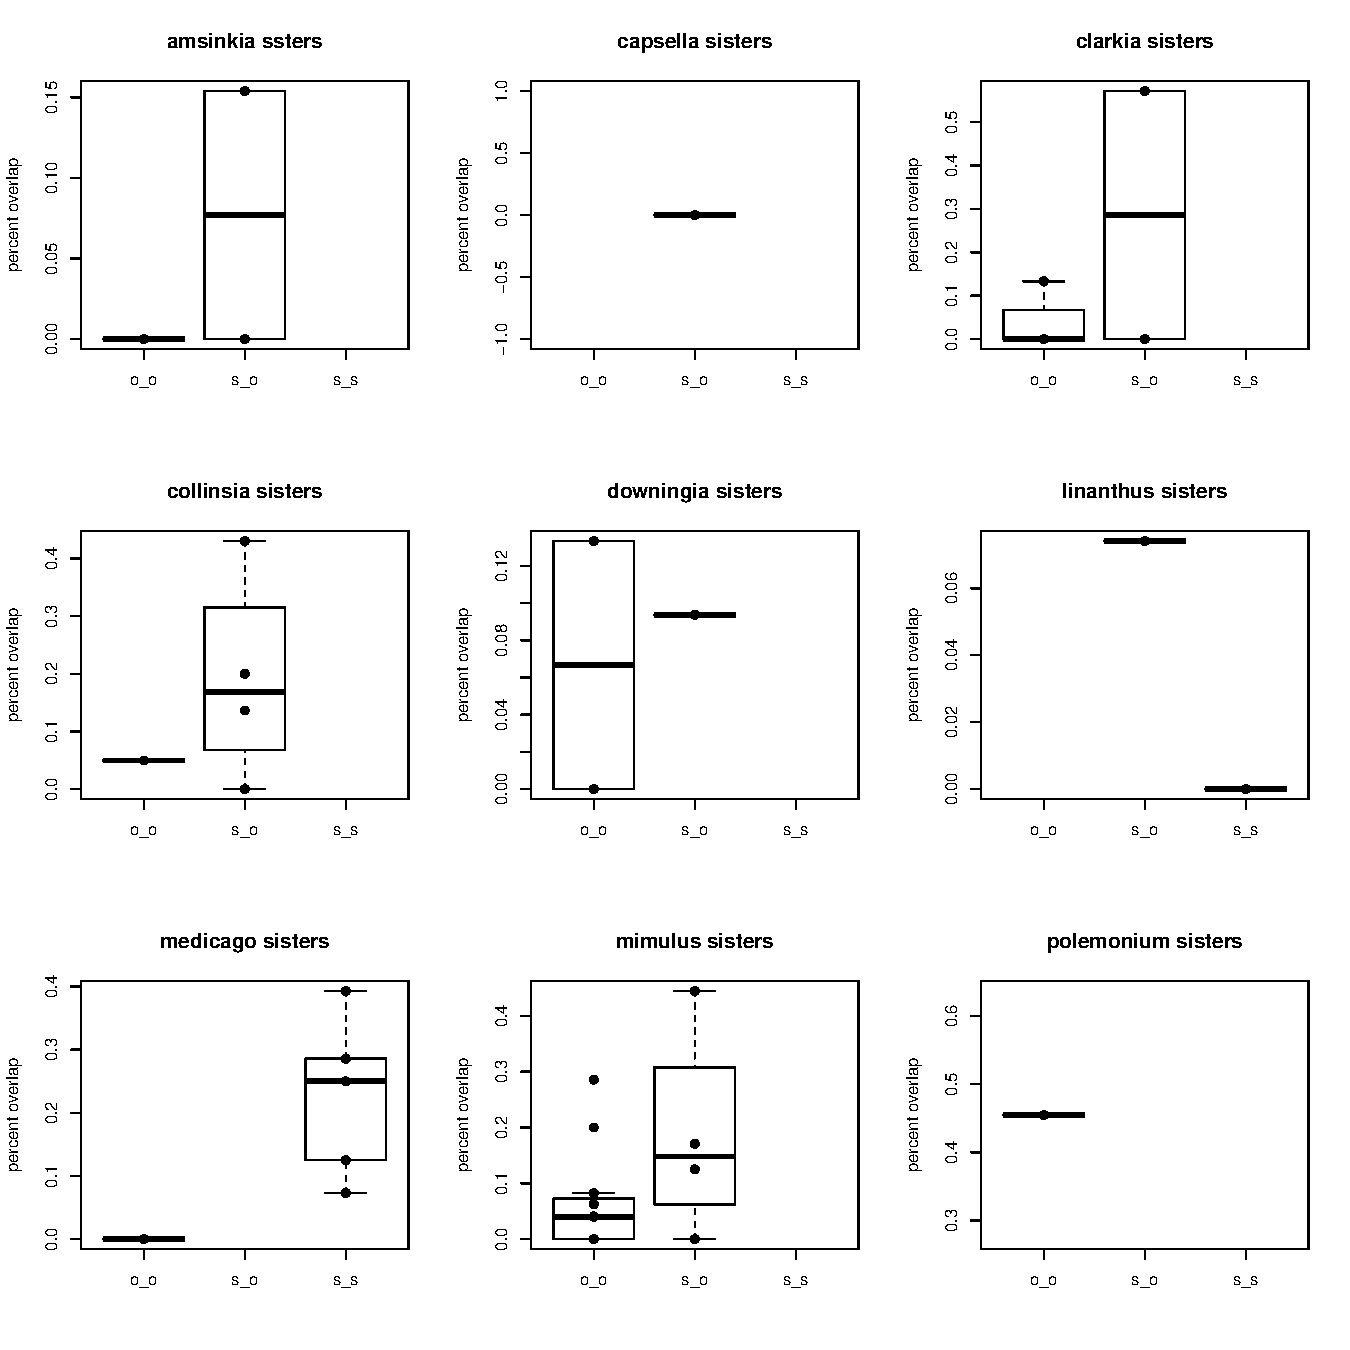
\includegraphics[width=1\textwidth]{sisters_fig008}
\end{figure}

\begin{figure}[h!]
\caption{Coarse scale sister pair co-occurrence. co-occurrence=overlap/min range.}
\centering
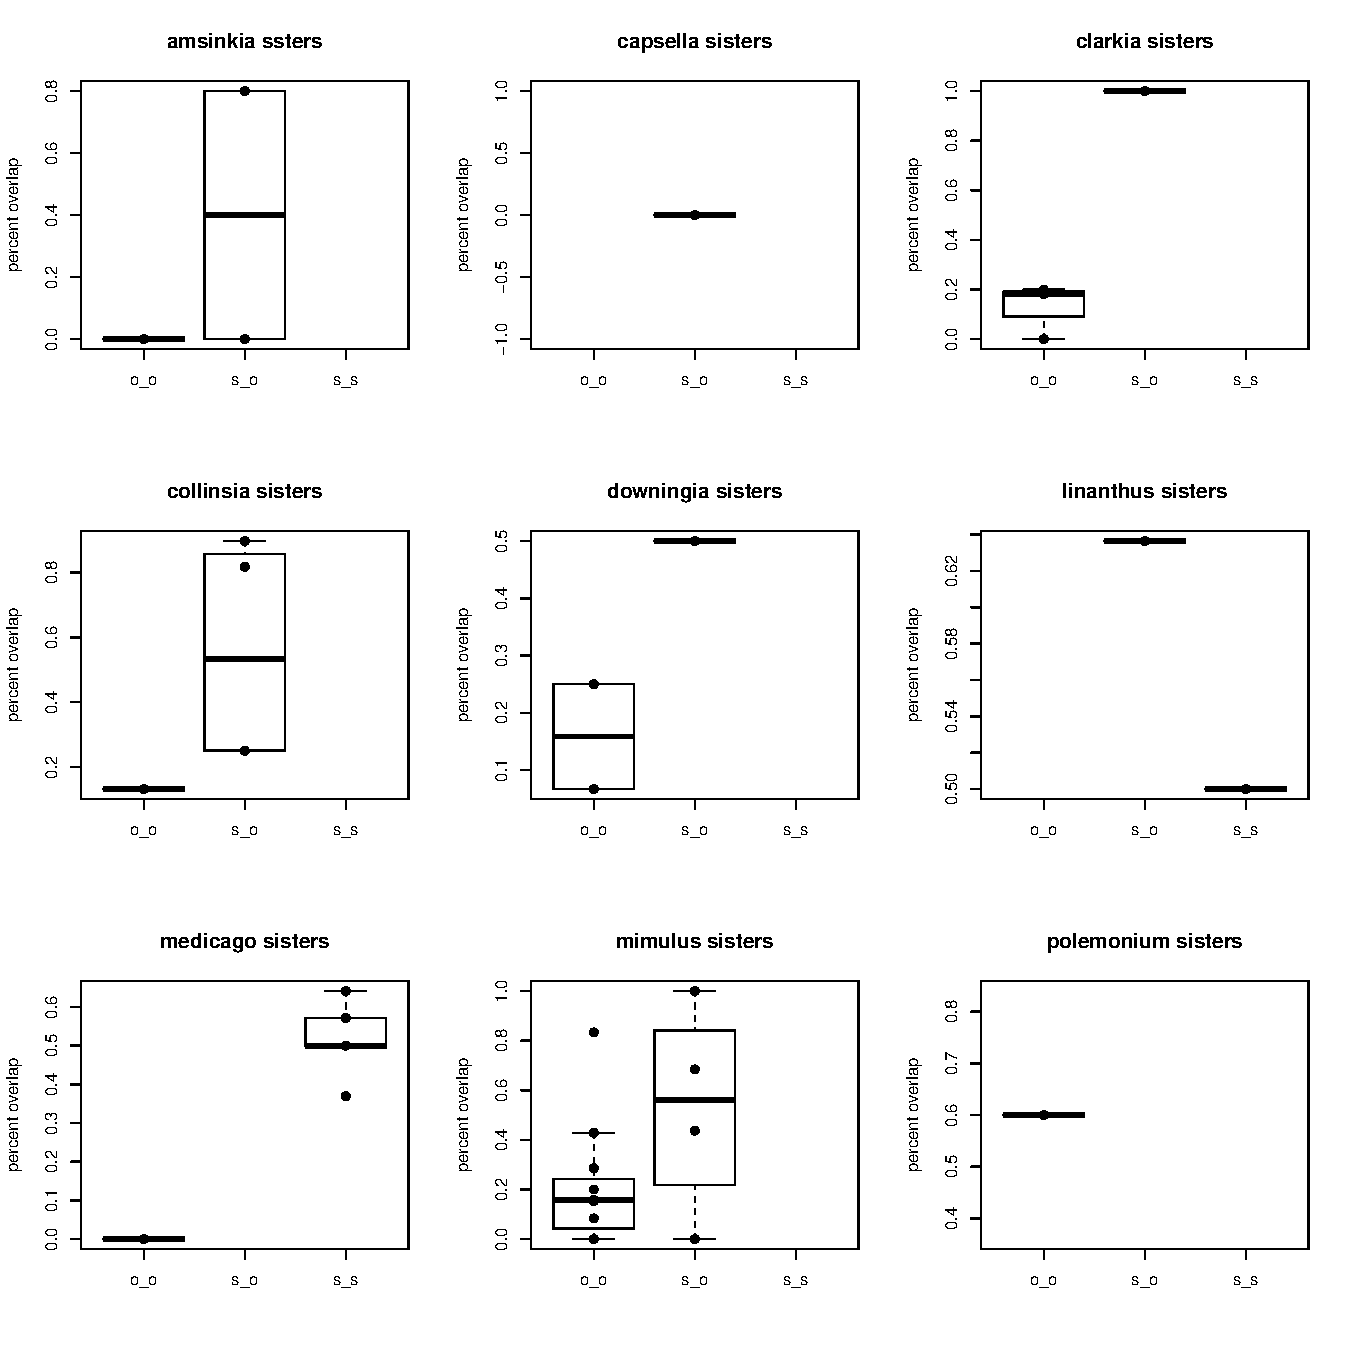
\includegraphics[width=1\textwidth]{sisters_fig5}
\end{figure}

\begin{figure}[h!]
\caption{Fine scale co-occurrence by node age - FT test. co-occurrence=overlap/min range}
\centering
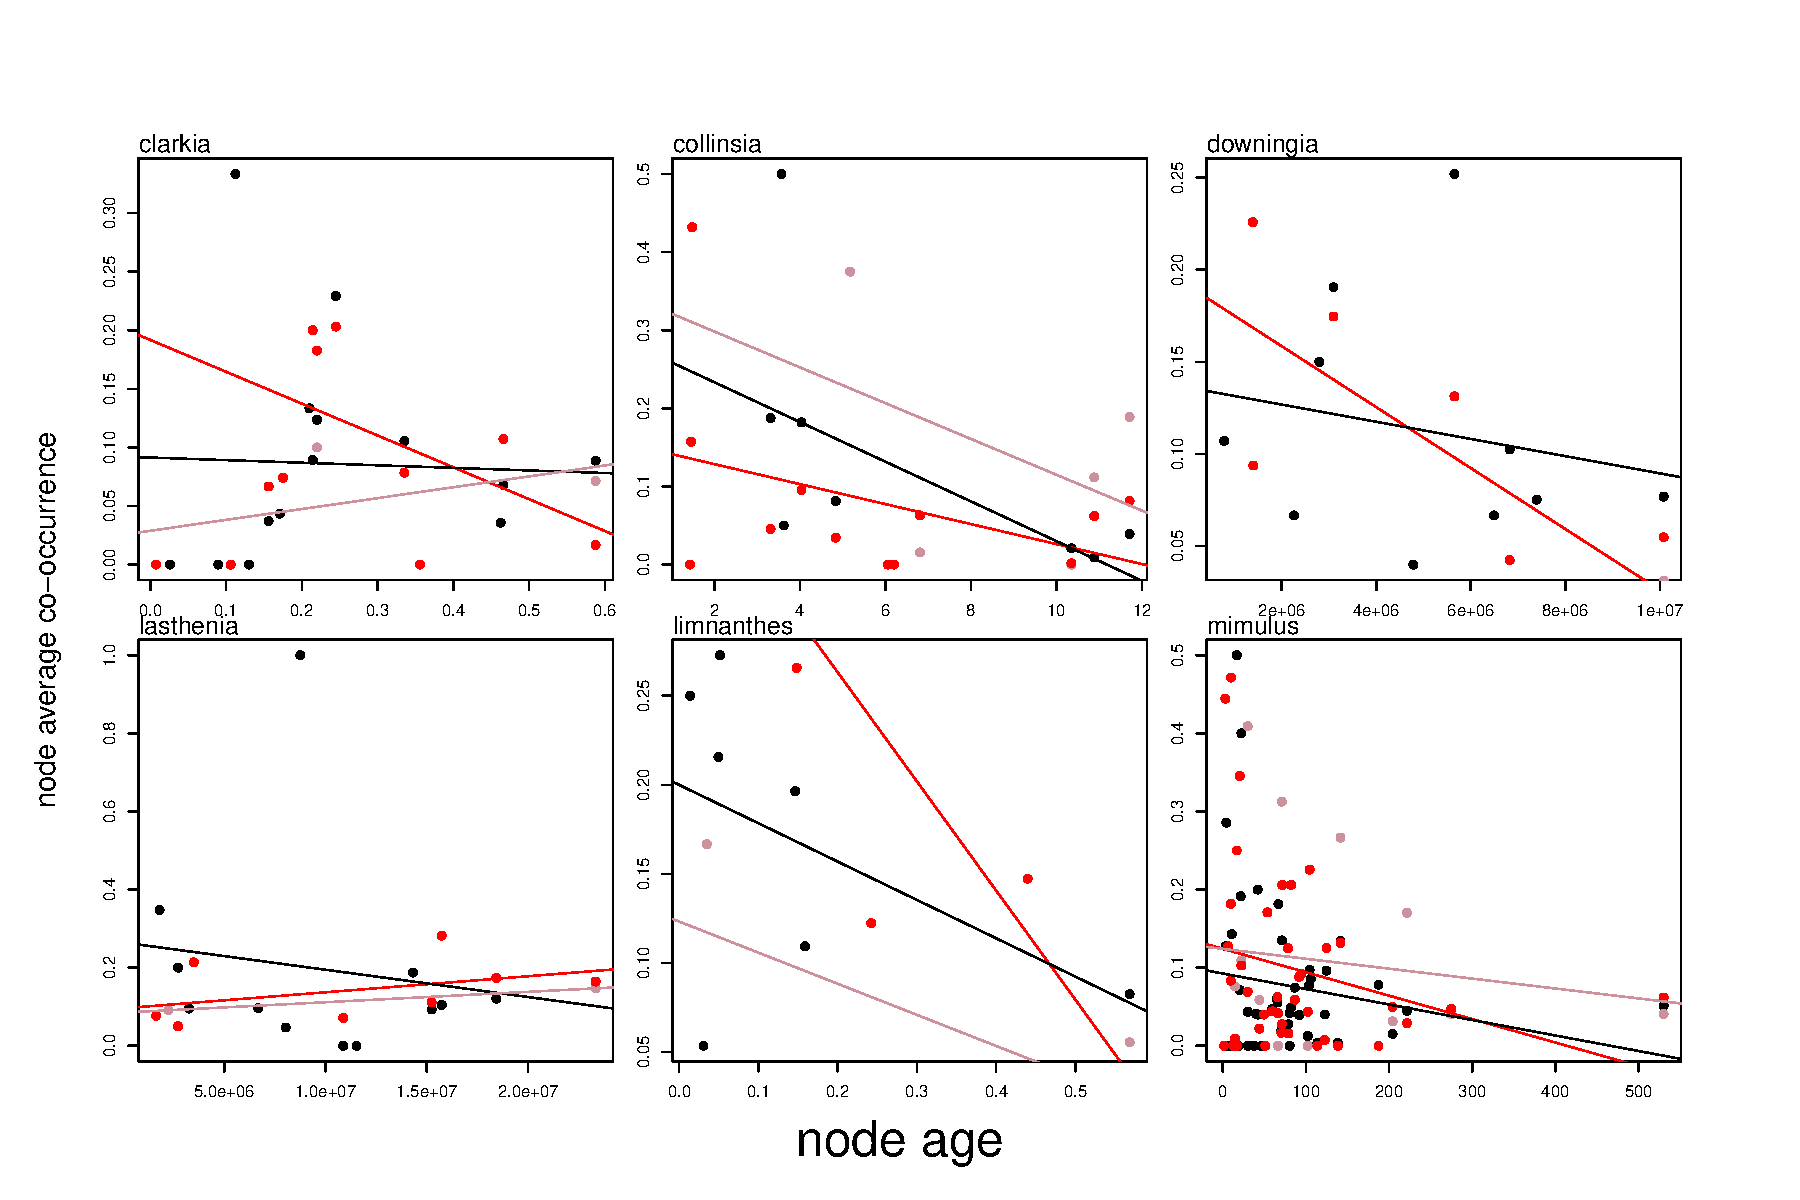
\includegraphics[width=0.8\textwidth]{overlap_age_FT_008_fig}
\end{figure}

\begin{figure}[h!]
\centering
\caption{Coarse scale co-occurrence by node age - FT test. co-occurrence=overlap/min range}
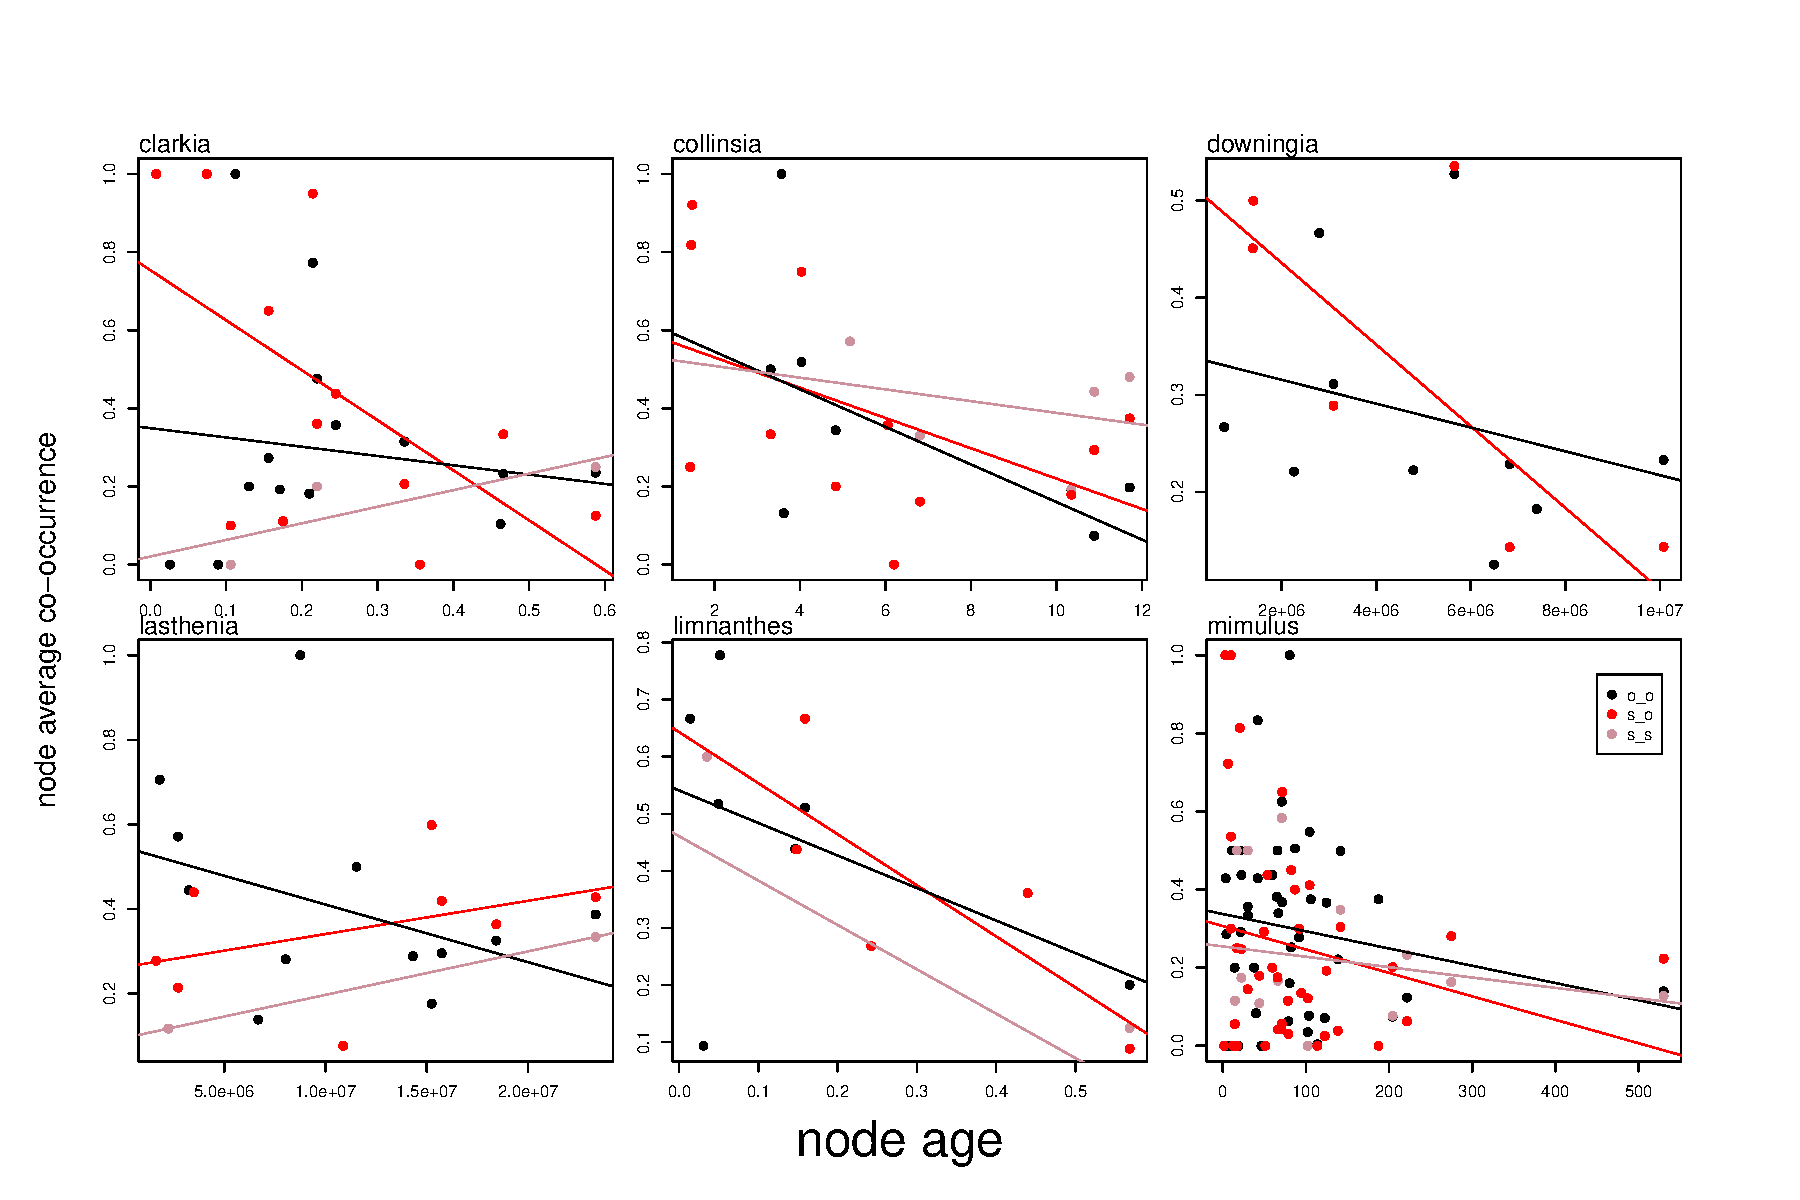
\includegraphics[width=0.8\textwidth]{overlap_age_FT_5_fig}
\end{figure}

\begin{figure}[h!]
 \caption{Fine scale co-occurrence by node age. co-occurrence=overlap/min range}
 \centering
 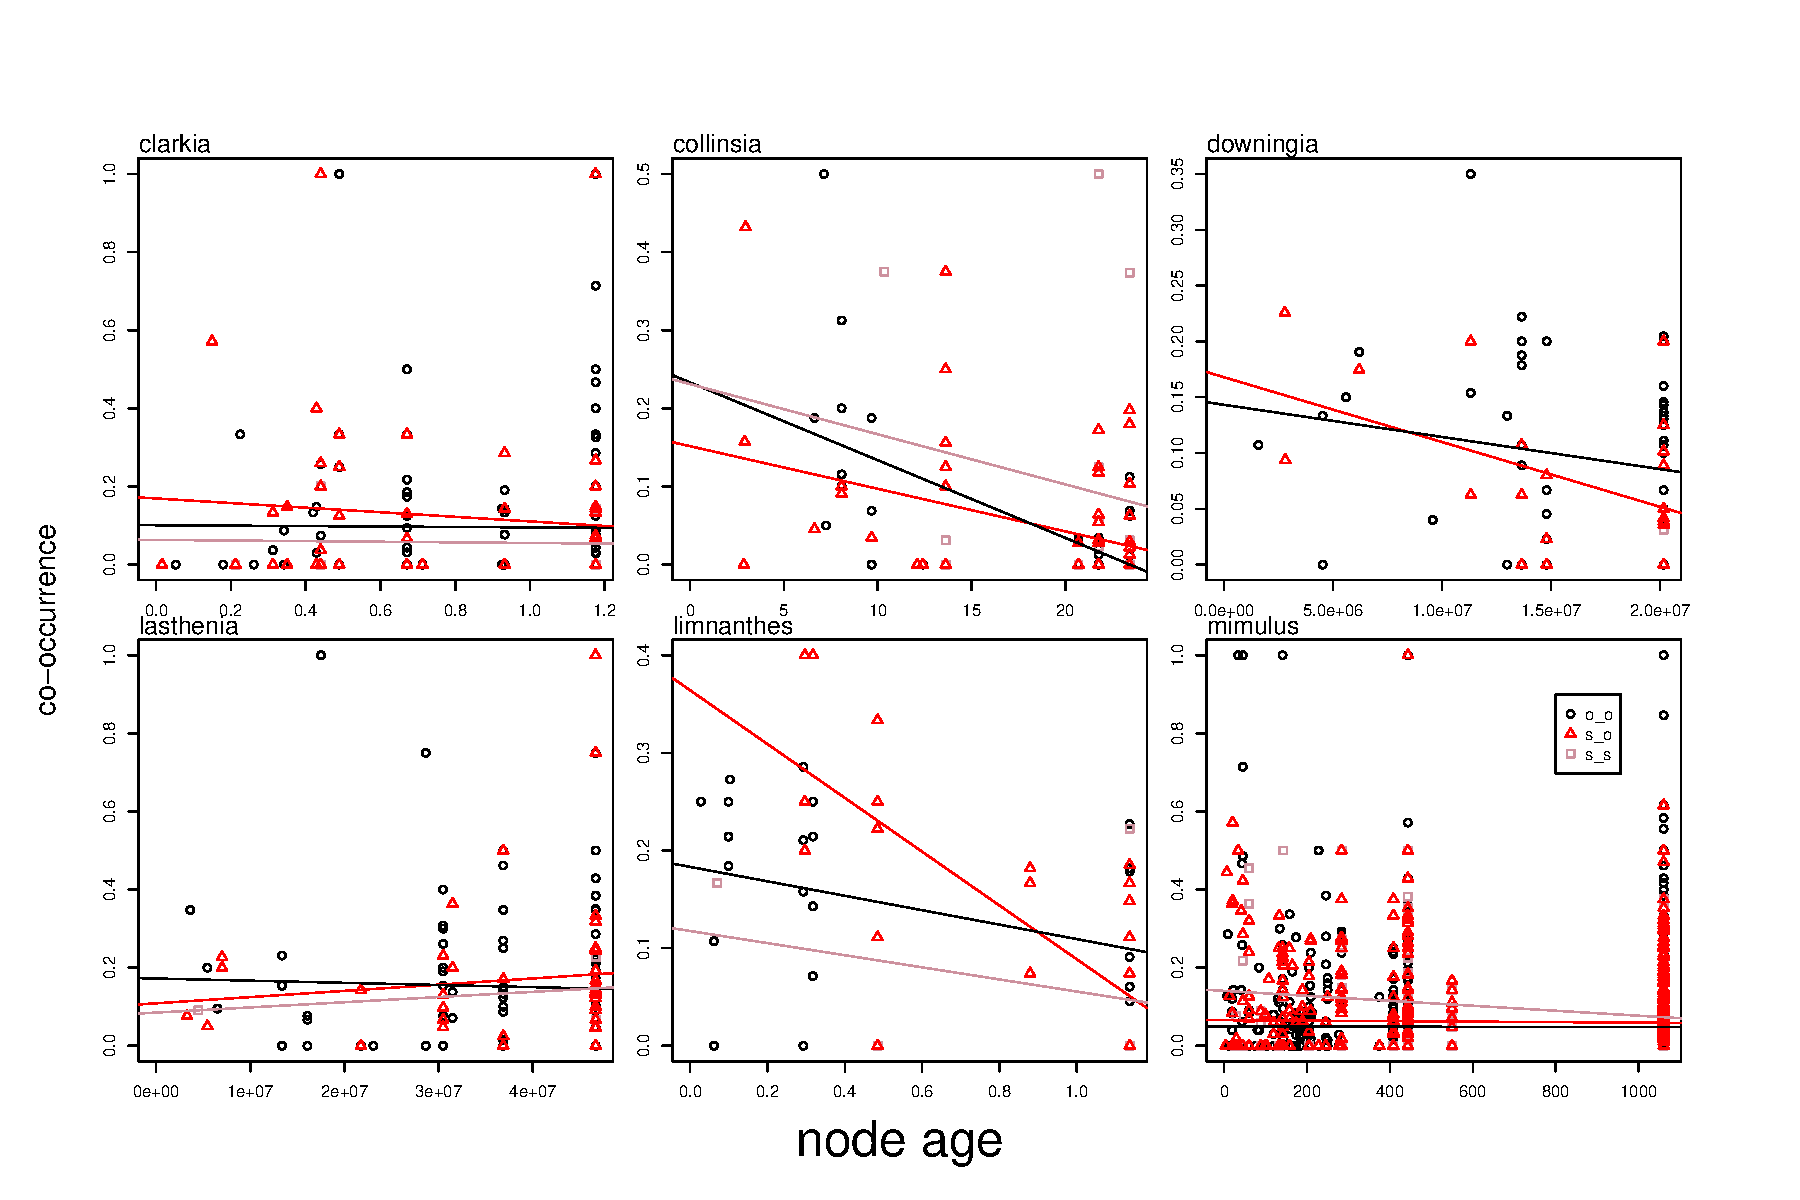
\includegraphics[width=0.8\textwidth]{overlap_age_008_fig}
\end{figure}

\begin{figure}[h!]
\centering
\caption{Coarse scale co-occurrence by node age. co-occurrence=overlap/min range}
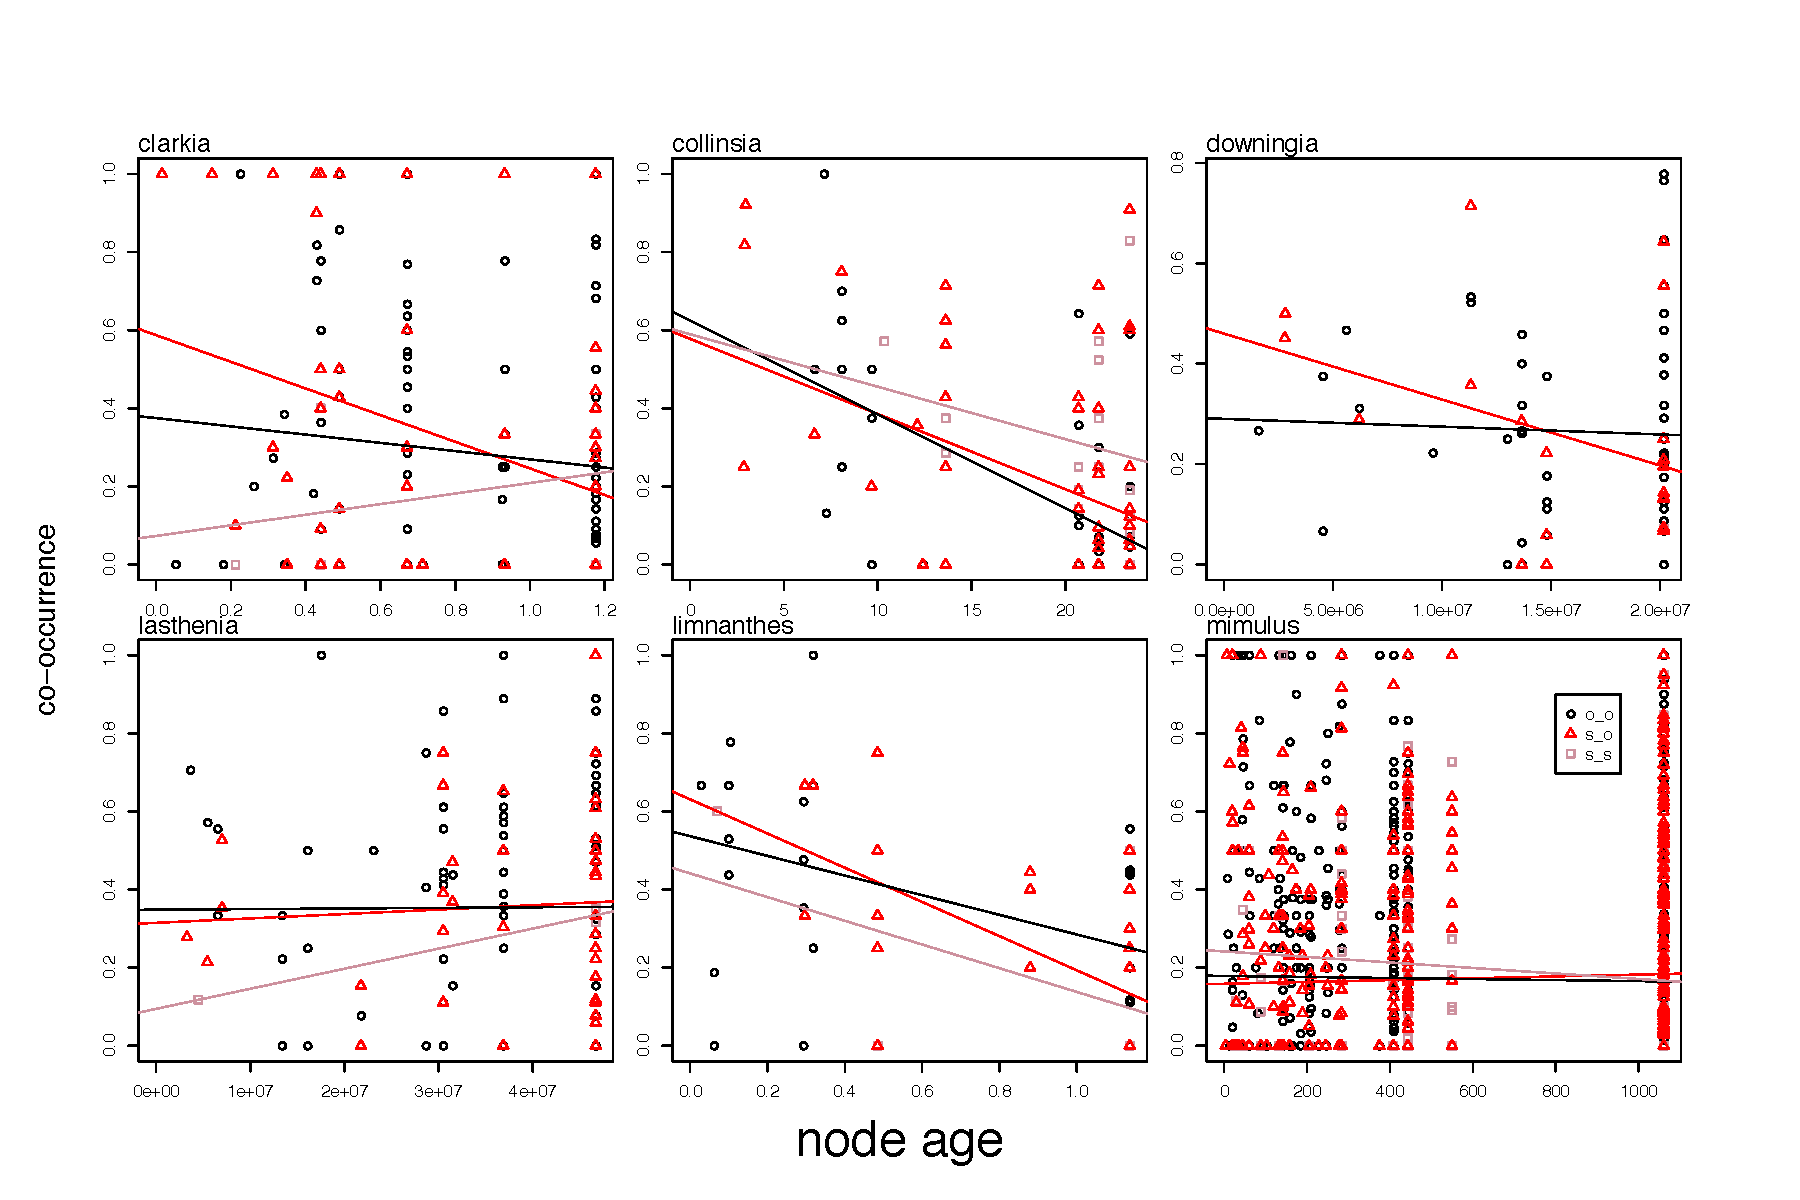
\includegraphics[width=0.8\textwidth]{overlap_age_5_fig}
\end{figure}

\begin{figure}[h!]
 \caption{Fine scale (s,o)o triplets: proportion(s,o co-occurrence $>$ o,o co-occurrence) by node age. co-occurrence=overlap/sister range}
 \centering
 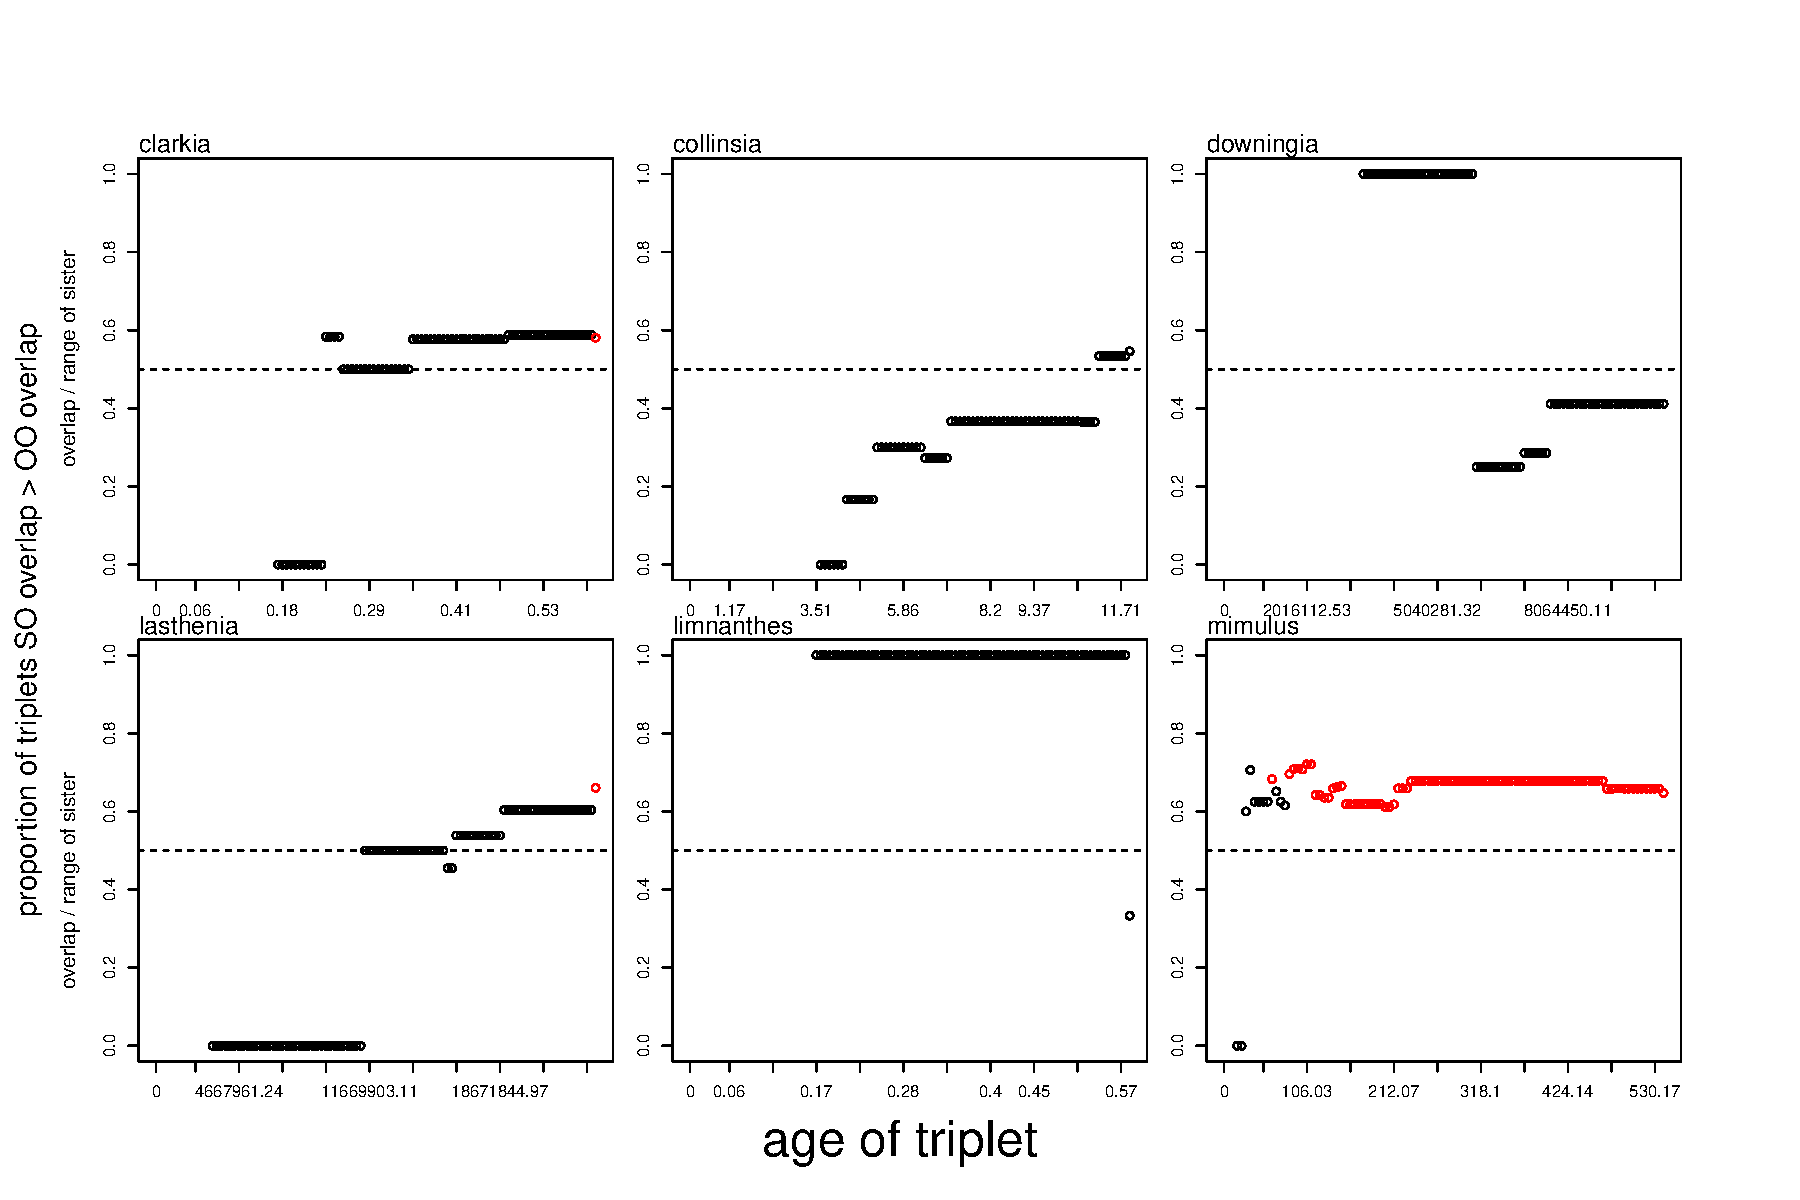
\includegraphics[width=0.8\textwidth]{triplets_signtest_res008}
\end{figure}

\begin{figure}[h!]
\centering
\caption{Coarse scale (s,o)o triplets: proportion(s,o co-occurrence $>$ o,o co-occurrence) by node age. co-occurrence=overlap/sister range}
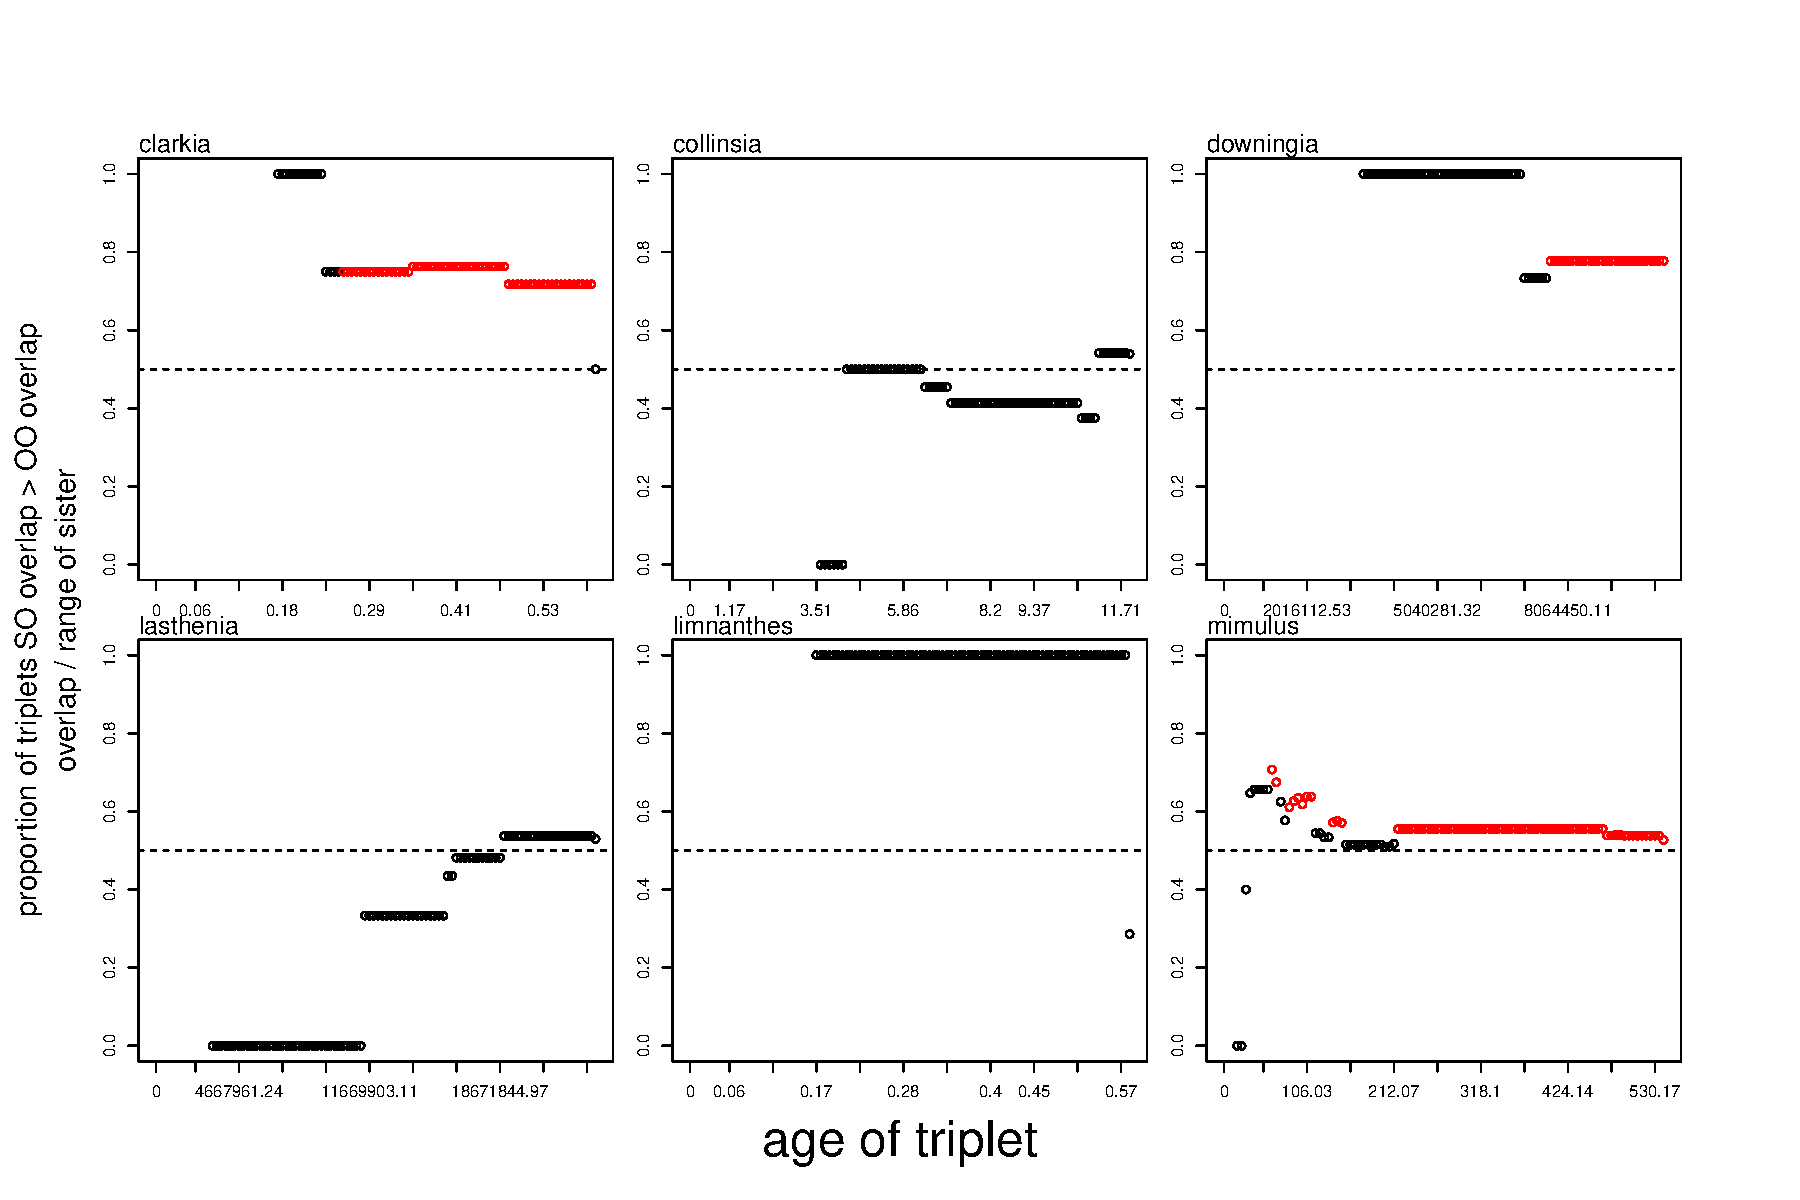
\includegraphics[width=0.8\textwidth]{triplets_signtest_res5}
\end{figure}

\begin{figure}[h!]
 \caption{Fine scale (s,o)o triplets: s,o co-occurrence $-$ o,o co-occurrence by node age. co-occurrence=overlap/sister range}
 \centering
 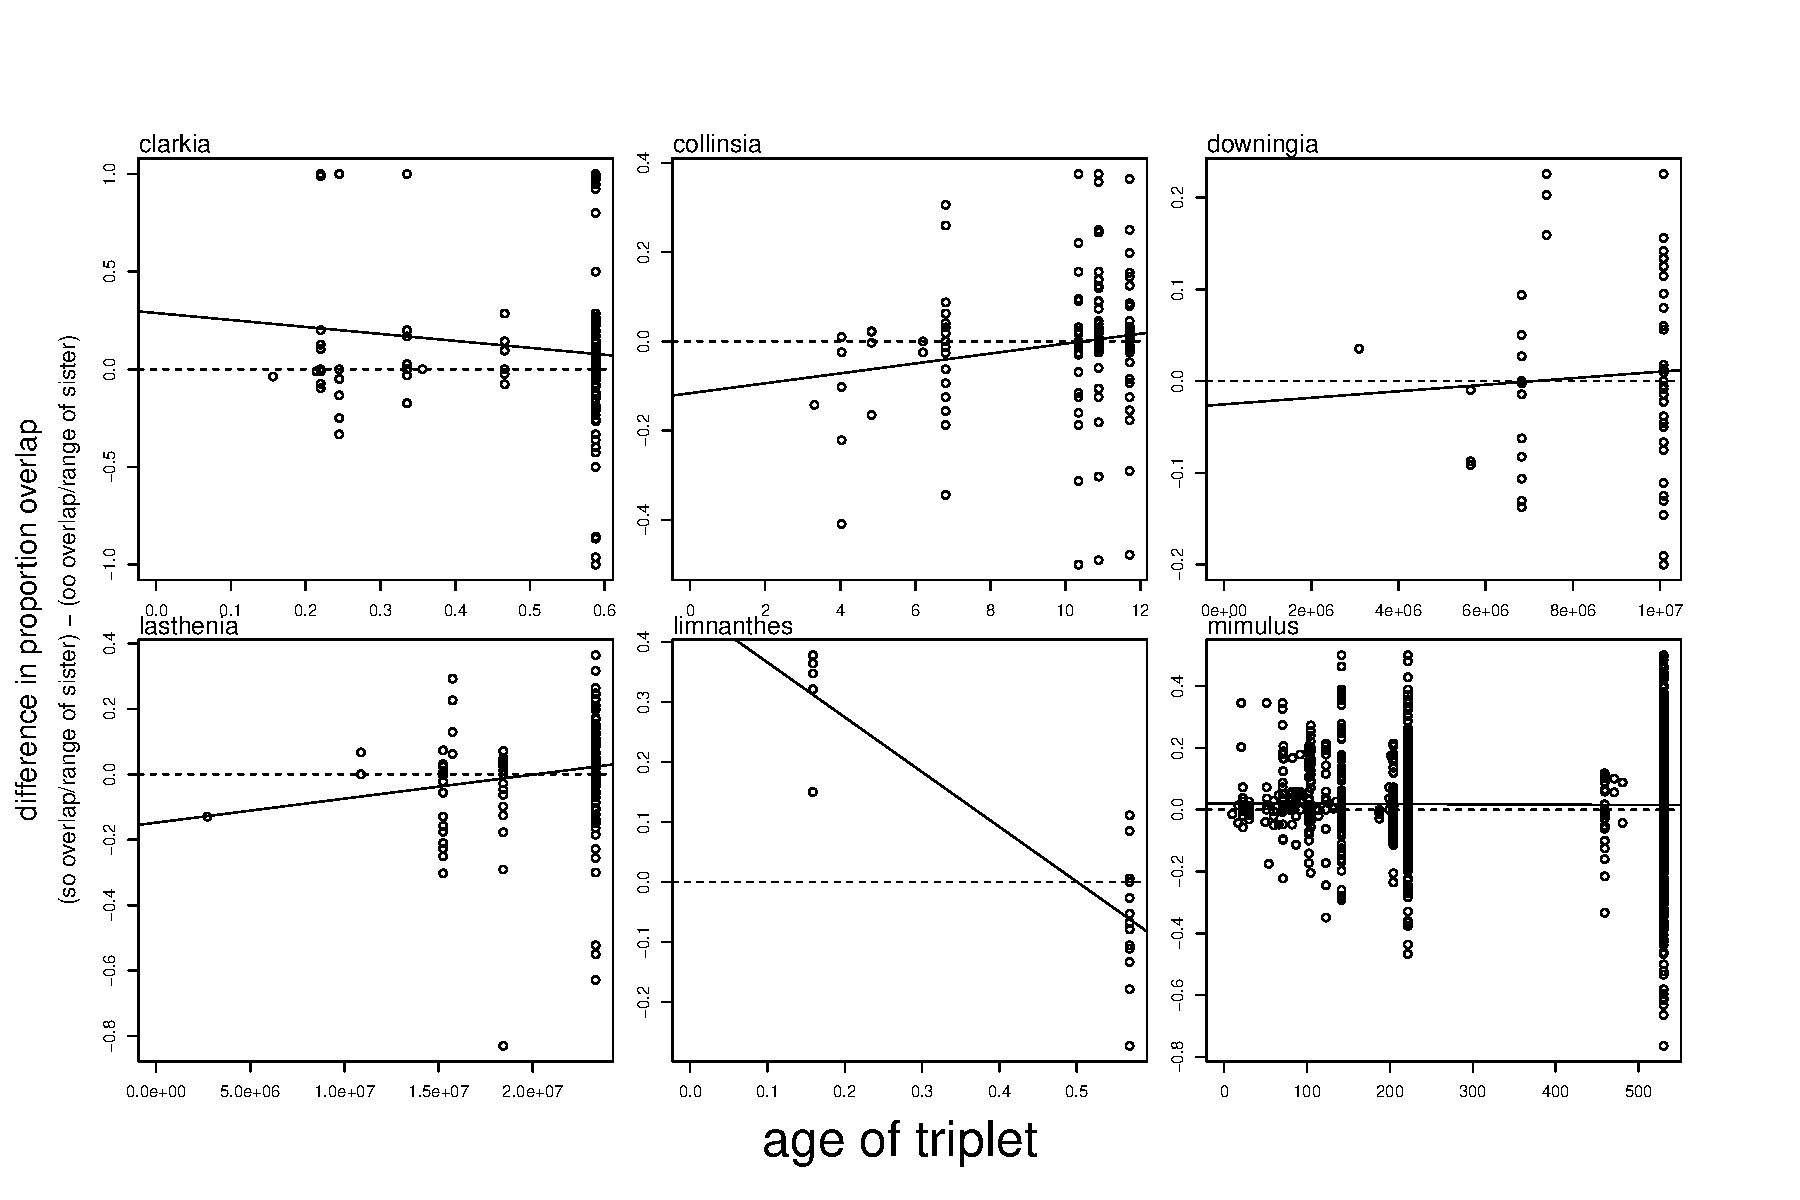
\includegraphics[width=0.8\textwidth]{tripletsAll008}
\end{figure}

\begin{figure}[h!]
\centering
\caption{Coarse scale (s,o)o triplets: s,o co-occurrence $-$ o,o co-occurrence by node age. co-occurrence=overlap/sister range}
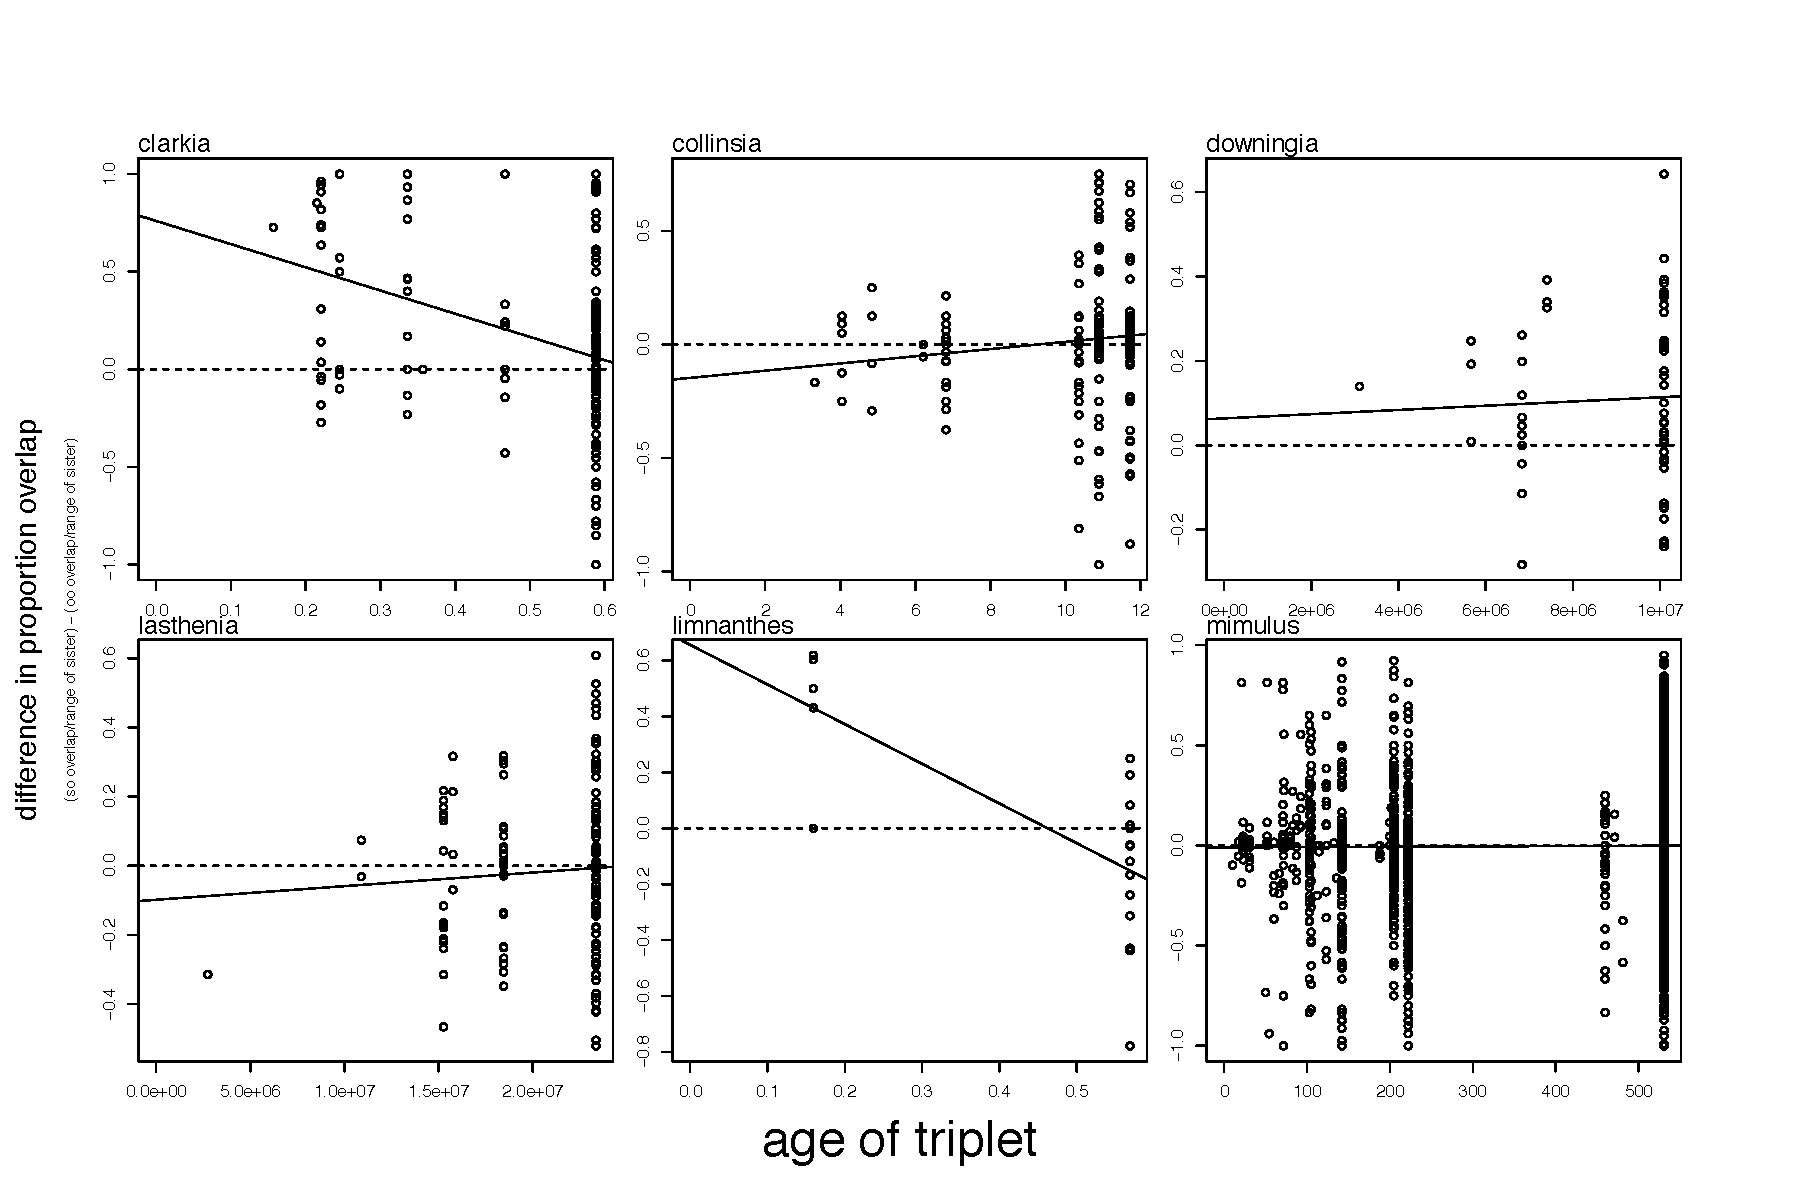
\includegraphics[width=0.8\textwidth]{tripletsAll5}
\end{figure}


% latex table generated in R 2.14.1 by xtable 1.6-0 package
% Thu May  1 15:08:33 2014
% latex table generated in R 2.14.1 by xtable 1.6-0 package
% Thu May  1 15:24:53 2014
\begin{table}[ht]
 \caption{Study clades}
\begin{center}
\begin{tabular}{|p{1cm}|p{2.5cm}|p{3cm}|p{3cm}|p{1cm}|p{1cm}|}
  \hline
 & Clade & Basis of Mating System & Basis of Phylogeny & Basis of Geographic Data & N species with complete data \\ 
  \hline
1 & Amsinckia & molecular and morphological &  & GBIF &  11 \\ 
  2 & Arapidopsis & molecular  &  & GBIF &   5 \\ 
  3 & Capsella & molecular  &  & GBIF &   3 \\ 
  4 & Clarkia & morphological and molecular &  & GBIF &  41 \\ 
  5 & Collinsia & morphological &  & GBIF &  19 \\ 
  6 & Downingia & morphological  &  & GBIF &  13 \\ 
  7 & Lasthenia & self incompatibility tests&  & GBIF &  19 \\ 
  8 & Leavenworthia & pers. Com. Herlihy &  & GBIF &   7 \\ 
  9 & Limnanthes & morphology, greenhouse study, molecular  &  & GBIF &  18 \\ 
  10 & Linanthus & self incompatibility tests &  & GBIF &  10 \\ 
  11 & Medicago &  previous reports and greenhouse &  & GBIF &  47 \\ 
  12 & Mimulus & Morphological and molecular &  & GBIF &  75 \\ 
  13 & Polemonium & Greenhouse crosses and morphology &  & GBIF &   6 \\ 
   \hline
\end{tabular}
\end{center}
\end{table}



\end{document}
